\let\negmedspace\undefined
\let\negthickspace\undefined
\documentclass[journal]{IEEEtran}
\usepackage[a4paper, margin=10mm, onecolumn]{geometry}
\usepackage{lmodern} % Ensure lmodern is loaded for pdflatex
\usepackage{tfrupee} % Include tfrupee package

\setlength{\headheight}{1cm} % Set the height of the header box
\setlength{\headsep}{0mm}  % Set the distance between the header box and the top of the text

\usepackage{gvv-book}
\usepackage{gvv}
\usepackage{cite}
\usepackage{amsmath,amssymb,amsfonts,amsthm}
\usepackage{algorithmic}
\usepackage{graphicx}
\usepackage{float}
\usepackage{textcomp}
\usepackage{xcolor}
\usepackage{txfonts}
\usepackage{listings}
\usepackage{enumitem}
\usepackage{mathtools}
\usepackage{gensymb}
\usepackage{comment}
\usepackage[breaklinks=true]{hyperref}
\usepackage{tkz-euclide} 
\usepackage{listings}
% \usepackage{gvv}                                        
\def\inputGnumericTable{}                                 
\usepackage[latin1]{inputenc}                                
\usepackage{color}                                            
\usepackage{array}                                            
\usepackage{longtable}                                       
\usepackage{calc}                                             
\usepackage{multirow}                                         
\usepackage{hhline}                                           
\usepackage{ifthen}                                           
\usepackage{lscape}
\usepackage{tikz}
\usetikzlibrary{patterns}

\begin{document}

\bibliographystyle{IEEEtran}
\vspace{3cm}

\title{1.1.6.14}
\author{EE25BTECH11064 - Yojit Manral}

\maketitle
% \maketitle
% \newpage
% \bigskip
{\let\newpage\relax\maketitle}
\renewcommand{\thefigure}{\theenumi}
\renewcommand{\thetable}{\theenumi}
\setlength{\intextsep}{10pt} % Space between text and float

\textbf{Question:}\\
Points $\Vec{A}$$\brak{3,1}$, $\Vec{B}$$\brak{12,-2}$ and $\Vec{C}$$\brak{0,2}$ cannot be the vertices of a triangle.\\

\textbf{Solution:}\\
\begin{table}[h!]    
  \centering
  \begin{tabular}[12pt]{ |c| c|}
    \hline
    \textbf{Points} & \textbf{Name}\\ 
    \hline
	\myvec{7\\10} & Point $\Vec{A}$ \\
    \hline 
	\myvec{-2\\5} & Point $\Vec{B}$\\
    \hline
	\myvec{3\\4} & Point $\Vec{C}$\\
    \hline
\end{tabular}
  \caption{List of Points}
  \label{Table_1}
\end{table}\\

$\rightarrow$ Any 3 points form a triangle if the rank of co-linearity matrix is not equal to 1, in which case they become collinear. For the rank of a matrix to be 1, the number of rows with non-zero entries should be 1 in row echelon form. \\
$\rightarrow$ The co-linearity matrix is given by,
\begin{align}
\myvec{\vec{B}-\vec{A} & \vec{C}-\vec{A}}^T = \myvec{9 & -3 \\ -3 & 1}\\
\notag
\end{align}
\begin{align}
\myvec{9 & -3 \\ -3 & 1}
&\xrightarrow{R_2 \leftrightarrow R_1 + 3R_2}
\myvec{9 & -3 \\ 0 & 0}\\
\notag
\end{align}
$\rightarrow$ The above matrix is in the row echelon form. Rank of the matrix in echelon form is the number of non-zero rows. Hence, rank of the above matrix is 1.\\
$\implies$ The given 3 points A, B, C are collinear. Thus, they cannot be part of a triangle.
\begin{figure}[h!]
   \centering
   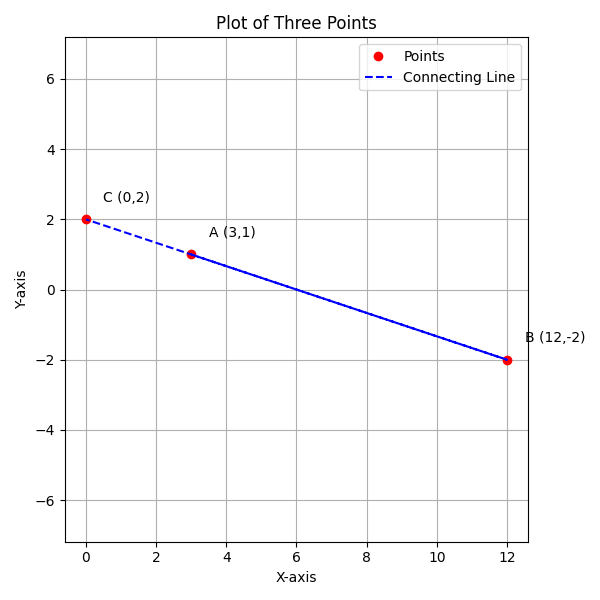
\includegraphics[width=0.5\linewidth]{figs/01.png}
   \caption{Plot of the points A, B, C}
   \label{Plot_1}
\end{figure}
\end{document}
